\chapter{Identity-Based Cryptography}\label{chp:ibc}
This chapter will present the concept of \gls{IBE} and \gls{IBS}, and why it is highly applicable to use this type of cryptography in \gls{NDN}. 
The possibilities to use the file synchronization module to do key distribution and revocation will be introduced.

\section{Concept}\label{ibc}
\gls{IBE} was first proposed by Shamir~\cite{DBLP:conf/crypto/Shamir84} in 1984. 
Shamir proposed a scheme for \gls{IBS}, but not a scheme for \gls{IBE}. 
The concept of \gls{IBE} builds upon every user having an \gls{ID} that is used as the \gls{PK}. 
This \gls{ID} can be anything, i.e. email, phone number, \gls{SSN}, or a \gls{name} (\autoref{name}).
The \gls{SK} that is extracted from the \gls{ID} is issued by a \gls{TTP}.
Notice that if every user could have created their own \gls{SK}, then so could anybody else with the same computational power, since the user does not obtain any ``privileged'' information about its \gls{ID}~\cite{Bidgoli06}.
This eliminates the need of certificates because the \gls{SK} allocation itself is a verfication by the \gls{TTP}.
The \gls{IBE} implementation remained unsolved until 2001, when Dan Boneh and Matthew K. Franklin proposed~\cite{DBLP:conf/crypto/BonehF01}.
However the scheme has only been shown to be secure within the random oracles model~\cite{DBLP:journals/iacr/Waters04}, hence less practical.

\gls{IBE} is based on performing asymmetric encryption with a publicly know \gls{ID} working as the \gls{PK}.
As seen in~\autoref{eq:mapping-id-name-pk}, the \gls{ID} can be a \gls{name} (e.g. ``/ndn/no/ntnu/haakon'').
Hence the \gls{name} becomes the \gls{PK} (from now referred to as \gls{ID}).
Therefore \gls{IBE} is highly applicable to \gls{NDN}.

\begin{equation}\label{eq:mapping-id-name-pk}
ID_{device} = PK_{device} = Name_{device}
\end{equation}

In \gls{IBE} there is a \gls{TTP} that is called \gls{PKG}.
The \gls{PKG}s task is to extract a secret key given an \gls{ID} and provide public parameters (\gls{MPK}) needed for performing encryption, decryption, signing and verifying. In~\autoref{fig:pkg_functions} the \gls{IBC} methods is illustrated in practice. 
First the \texttt{PKG} runs \texttt{Setup()}. 
\texttt{device1} can then request a \texttt{SK} by sending \texttt{ID\textsubscript{d1}} to the \texttt{PKG}. 
In return the \texttt{device1} receives the \texttt{SK\textsubscript{d1}} as well as the \texttt{MPK\textsubscript{PKG}}.
\texttt{device2}, which is already a part of the trust domain, sends a signed request for \gls{data} to \texttt{device1}. 
\texttt{device1} verifies the signature and responds to the request with a signed, encrypted content.
\texttt{device0}, which do not have a \gls{SK} generated from the \texttt{PKG} and thus is not a part of the trust domain, sends a request to \texttt{device1} that is declined.

\begin{enumerate}\label{ibc-methods}
  \item \texttt{Setup()} generates a key pair, \gls{MPK} and \gls{MSK}. 
  These keys are used by only the \gls{PKG} to extracting secret keys, encryption and decryption.
  \item \texttt{Extract(MPK\textsubscript{PKG}, MSK\textsubscript{PKG}, ID\textsubscript{device})} generates a secret key from a given ID. 
  \item \texttt{Encrypt(MPK\textsubscript{PKG}, ID\textsubscript{device}, message)} encrypts the message.
  \item \texttt{Decrypt(MPK\textsubscript{PKG}, SK\textsubscript{device}, cipher)} decrypts the cipher generated from the encryption.
  \item \texttt{Signing(MPK\textsubscript{PKG}, SK\textsubscript{device}, message)} signs a hash digest of the message (e.g. \gls{SHA1}).
  \item \texttt{Verify(MPK\textsubscript{PKG}, ID\textsubscript{device}, message, signature)} verifies the signature.
\end{enumerate}

\begin{figure}[ht]
  \centering
  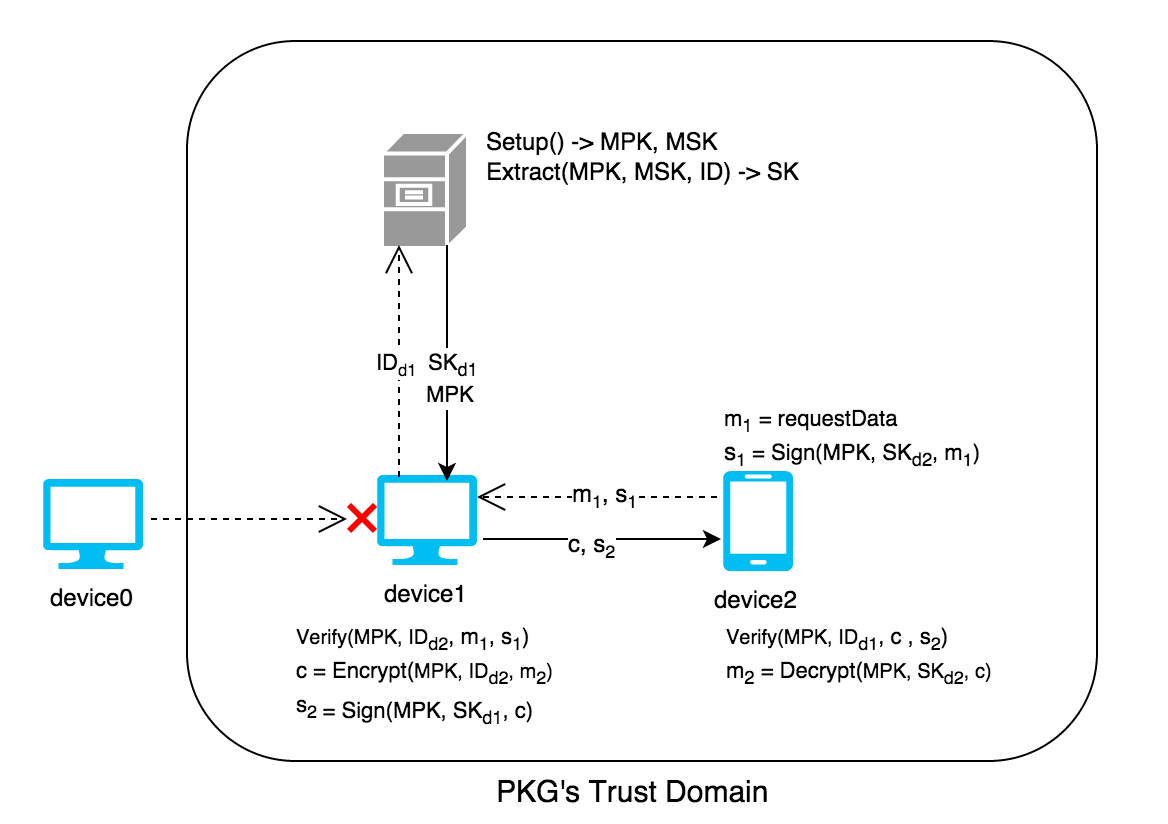
\includegraphics[width=1\textwidth]{pkg_functions.png}
  \caption{Methods of an IBC systems illustrated in practice.}
  \label{fig:pkg_functions}
\end{figure}

To encrypt a message with \gls{IBE}, the user encrypts a \gls{CEK} with the recipients \gls{ID}.
The user encrypts the message using the \gls{CEK} together with symmetric encryption~\cite[section 2.2.2]{rfc5408}, and sends both the encrypted \gls{CEK} and the encrypted content to the requester. 

Two main
Deploy a secure \gls{PKG}.
Identify each device before issuing \gls{SK}.

There are some drawbacks related to \gls{IBE} such as issues around trusting the \gls{PKG} considering that the \gls{PKG} generates all \gls{SK}s.  
If the \gls{PKG} is compromised by an adversary, the adversary will retrieve all \gls{SK}s belonging to the corresponding \gls{ID}. 
Suspicion of \gls{MITM}, where the \gls{PKG} is the adversary, can be a problem for users.
The same issue does however occur in Kerberos, which is a well recognized security system.
Initializing might also be a problem because to allocate \gls{SK}s, a secure channel has to be established. 
However, this is not a bugger problem than in existing networks. 
Pre-shared secrets or Diffie-Hellman key exchange might be a good solution.

\section{Secureness}\label{ibe-secureness}
When designing protocols in cryptography one first usually designs an ideal system where all parties have random oracle access, then proves the security.
A random oracle is like a ``black box'' that outputs truly random numbers.
Second, one replaces the oracle access with a hash function.
This gives an implementation of an ideal system in the real world, but without random oracles~\cite{DBLP:conf/ccs/BellareR93}. 
It is perfectly fine to make statements based on the ideal system, but debatable whether the same statements yields for the implementation in the real world.
Canetti et al. concluded that there exist secure schemes in the \textit{Random Oracle Model}, but for which any implementation of the random oracle results in insecure schemes~\cite{DBLP:journals/jacm/CanettiGH04}.
Boneh and Franklins \gls{IBE} scheme is only secure when using random oracles, and relies on elliptic curves~\cite{DBLP:conf/crypto/BonehF01}.

Following the \textit{Standard Model} one does not resort to the random oracle heuristic and does not rely on non-standard complexity assumptions.
Hence proving security in the standard model is preferably.
In 2004 Boneh and Boyen proposed a fully secure scheme in the standard model~\cite{DBLP:conf/crypto/BonehB04}.
However the scheme is not efficient. 

First practical scheme was introduces by Brent Waters~\cite{DBLP:journals/iacr/Waters04}.
But as David Naccache states in his paper~\cite{DBLP:journals/iacr/Naccache05}, Waters' scheme without random oracles introduces too large public parameters (164\gls{KB}!).
Naccache proves that he was able to construct a practical and fully secure scheme in the standard model based on the \gls{DBDH} assumption.
The scheme is a modification of Waters' scheme, but with public parameters of just a few \gls{KB} size.

Waters created a fully secure \gls{IBE} system with short parameters under \gls{simple_assumption} in 2009~\cite{DBLP:conf/crypto/Waters09}.

The complexity assumptions is based on bilinear maps.
Let $\mathbb{G}_1$ and $\mathbb{G}_2$ be groups of prime order \gls{p}, and $g$ be a generator of \gls{g}. 
We say that $\mathbb{G}$ has a bilinear map $e : \mathbb{G}_1 \times \mathbb{G}_2 \to \mathbb{G}_T$ if $e$ is efficiently computable, $e$ is bilinear, i.e. $e(g^a, g^b) = e(g, g)^{ab}$ (for all $a$ and $b$), and $e$ is non-degenerate, i.e. $e(g,g)\neq 1$.
For more details about bilinear maps and~\gls{BDH} used in \gls{IBE}, the reader is encouraged to take a look at~\cite{DBLP:conf/crypto/BonehF01,DBLP:journals/iacr/Naccache05}.

\section{Key Distribution}\label{key-distribution}
In traditional \gls{PKI}, each public key is signed by a certificate authority and the generated certificate is sent as a response over a secure channel then validated by the the client.
I want to make the certificate authority obsolete by distributing every \gls{ID}.
This can be done through the \gls{FSM} presented in~\autoref{file-sync}.
In~\autoref{fig:pkg_sync} we see that the \gls{PKG} multicasts the \gls{ID} list to all devices that have joined the trust domain.
Each device can verify the integrity and authenticity of the sync state \gls{data} and validate that the \gls{ID} list surely originates from its own \gls{PKG}, i.e. the distributor.
\begin{figure}[ht]
  \centering
  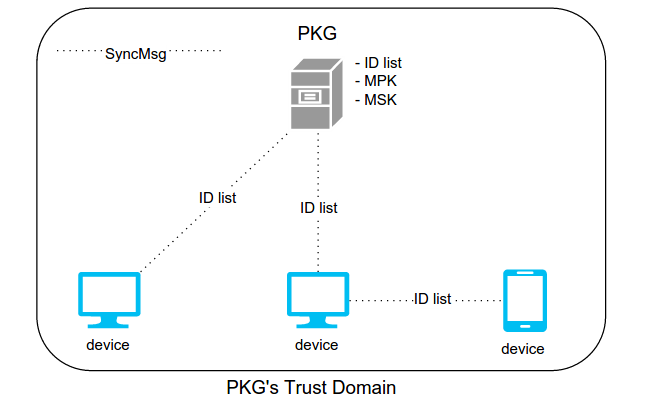
\includegraphics[width=1\textwidth]{pkg_sync.png}
  \caption{FSM with tree devices (subscribers) and a PKG (distributor).}
  \label{fig:pkg_sync}
\end{figure}

\todo{more existing solutions}

\section{Key Revocation}
Key revocation in systems are studied well in traditional \gls{PKI}.
However, few alternatives to revocation schemes in \gls{IBE} \gls{PKI} have been proposed.
One suggestion is to allocate secret keys with the \gls{ID} combined with some sort of date, e.g. month-year or just year~\cite[section 1.1.1]{DBLP:conf/crypto/BonehF01}. 
In this alternative a user has to renew its secret key each time the date changes, i.e. either the month or the year depending on the date format.
The problem with this revocation solution is that it can be cumbersome for the \gls{PKG}.
Boldyreva et al. proposes a revocation scheme~\cite{DBLP:journals/iacr/BoldyrevaGK12} based on efficient key-update, which makes the workload for the \gls{PKG} a lot easier. 
This scheme was only proven secure in the selective-ID setting where adversaries can attack an \gls{ID} given they choose which one at the beginning of the game.
The work done by Beno\^{i}t Libert and Damien Vergnaud in~\cite{DBLP:conf/ctrsa/LibertV09} solves this problem. 
However, efficiently delegating both the key generation and revocation functionalities was a problem left open.
Jae Hong Seo and Keita Emura solves this in~\cite{DBLP:journals/iacr/SeoE13a}.

If a key is compromised, we want to revoke the key immediately letting everybody know that this specific \gls{ID} has been revoked. 
One problem with key revocation is that there is no way of revoking this key, and thus the \gls{ID} has to be changed and distributed. 
However, a partially revocation can be sufficient in some networks. 
By partially, I do not mean revoking the private key, but rather only distributing the new public key (i.e. \gls{ID}) to every node in the trust domain.
In short, the compromised key should be removed from a distributed ID-list and the list containing only valid \gls{ID}s should be disseminated.
With the \gls{FSM}, the list is distributed automatically when updated, and only a \gls{DoS} attack together with a compromised key would make the system vulnerable. 
On the other side, some periodic renewal might be necessary because it is not always known that a key has been compromised.
